\documentclass[10pt]{article}
\usepackage[document]{ragged2e}
\usepackage{multicol}
\usepackage[margin=1in]{geometry}
\usepackage{titlesec}
\usepackage{fancyhdr}
\usepackage{graphicx}
\graphicspath{ {./images/} }
\usepackage[justification=centering]{caption}
\captionsetup[subfigure]{justification=centering}
\captionsetup[figure]{justification=centering}
\usepackage{subcaption}
\usepackage{float}


\pagestyle{fancy}
\fancyhf{}
\fancyfoot[R]{Page. \thepage}
\fancypagestyle{plain}{
    \renewcommand{\headrulewidth}{0pt}
    \fancyhf{}
    \fancyfoot[R]{Page. \thepage}
}

\setlength{\parindent}{0em}
\setlength{\parskip}{1em}
\titlespacing*{\section}{0pt}{0.2em}{0.5em}
\titlespacing*{\subsection}{0pt}{0.2em}{0.2em}
\titlespacing*{\subsubsection}{0pt}{0.2em}{0.2em}


\title{Checkpoint 5: Natural Language Processing}
\author{The Freedom Deer: Tianchang Li, Hualiang Qin, Qingwei Lan}

\begin{document}
\maketitle


In this checkpoint, we extended one of our previous exploratory findings which showed considerably more cross-race cases in use of force, meaning that the police officer and subject involved are from different race groups, than same-race cases. Here, we are interested in investigating the role race plays in police misconduct. 

Specifically, we hypothesized a linear regression model where:

\begin{centering}
Severity of a misconduct $\sim$ the heat / emergency of an accusation + race of two parties + other factors
\end{centering}

In plain words, we hypothesized that how severe a police misconduct is depends on how necessary it is given the accusation scenario, the race of police officer and subject, and some other factors. To implement this model, we extracted two specific allegations as our dependent variable, one from non-use-of-force category (``Inadequate / Failure To Provide Service") and the other from use-of-force category (``Excessive Force / On Duty - Injury"). We performed a sentimental analysis on the summary of each allegation based on a pre-trained model to get a sentimental score for each accusation scenario. We use the negativeness of each score to represent the heat/emergency of a scenario. The other factors that we can’t exhaust goes into the residual.

This is to say that, by looking at the statistical significance of race variable(s), we assessed whether using force is escalated by certain race compositions, controlling for the heat/emergency and other factors.


\section{Regression on police officers’ race and subjects' race}

We firstly run a regression with both officers’ race and subjects’ race to see how each of them influences use of force. 

Some details in manipulating the input data: we cast the lighter misconduct into 0 and heavier misconduct into 1 to represent the severity of misconduct; we also grouped all the officers’ race other than white into ‘other’ and grouped all the subjects’ race other than black into ‘other’. This is based on our previous findings that the majority of officers are white and the majority of subjects are black.

We obtained the following output:

\begin{figure}[H]
\centering
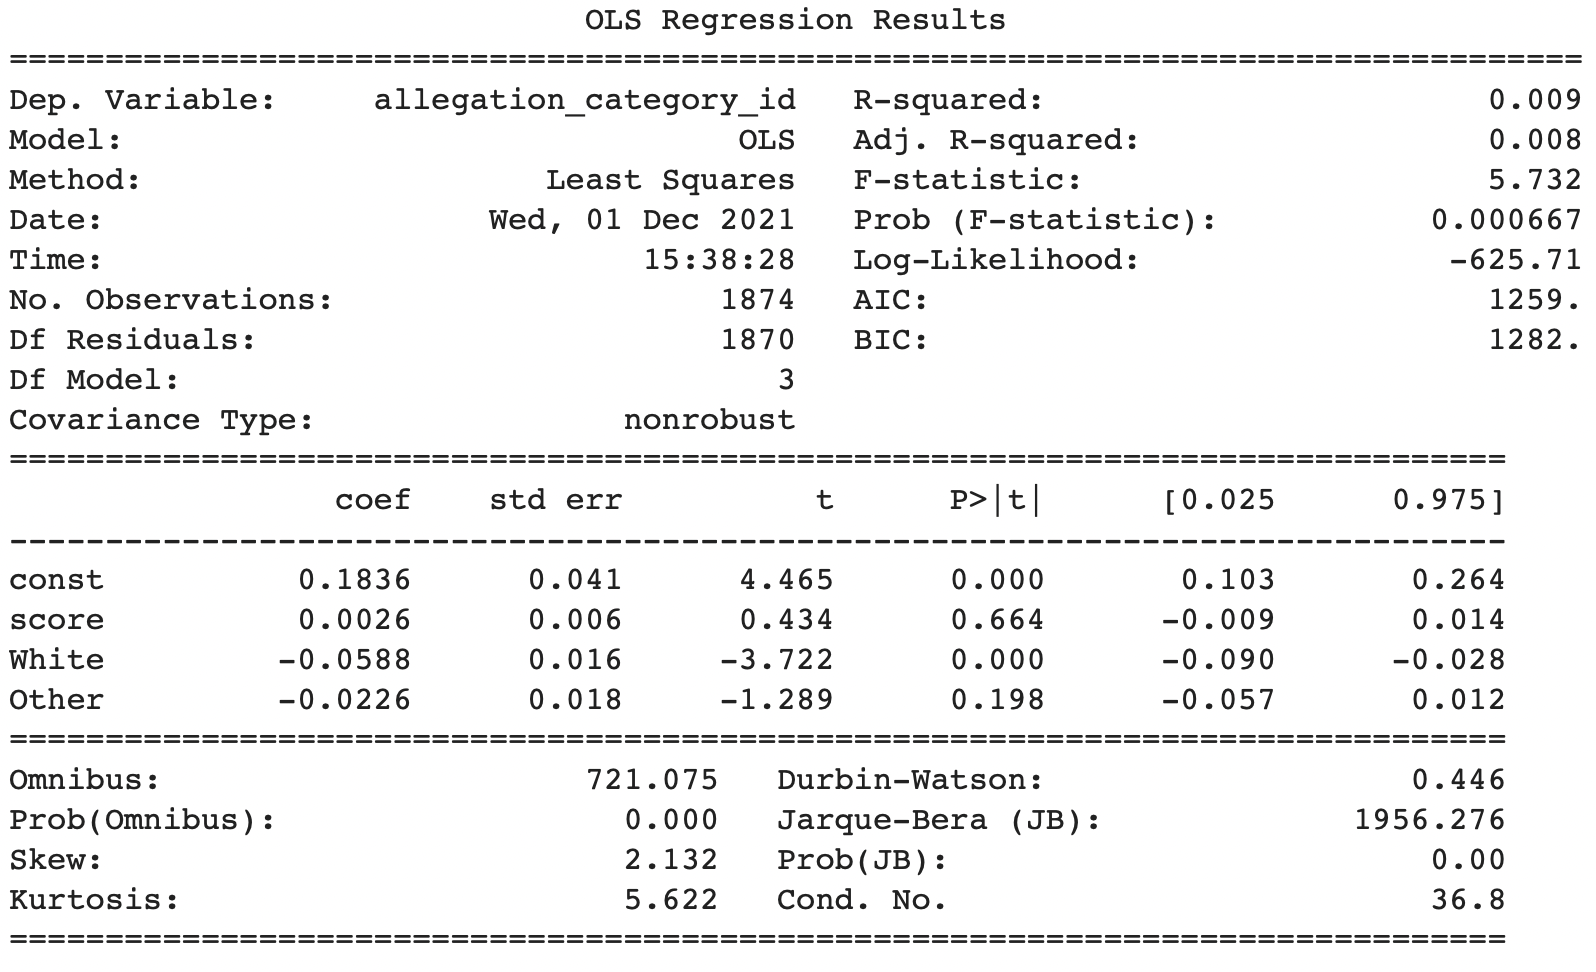
\includegraphics[width=\textwidth]{regression1}
\end{figure}


Looking at the table, one can see that the sentimental scores predict the severity of misconduct in the correct direction, although not significant. Also, being non-white is a statistically significant factor for a police officer to use force, while being black is a factor for a subject to experience force. Although the latter finding is not significant, we only used close to 2,000 cases here due to the limit of run time. With more samples, it might show significance. 

We should keep in mind that the findings are potentially subject to the undesirable features of the data, including the extremely unbalanced on racial composition in both officers and subjects and the biases going into alleging officers’ from different race groups differently.



\section{Regression on cross-race variable}

We then run a regression on whether the officers and subjects being in different race groups escalate the police misconduct.

Similarly, some details in manipulating the input data: we again cast the lighter misconduct into 0 and heavier misconduct into 1 to represent the severity of misconduct; we created an extra variable for cross-race, 1 being cross-race cases and 0 being same-race cases. 

We obtained the following results:

\begin{figure}[H]
\centering
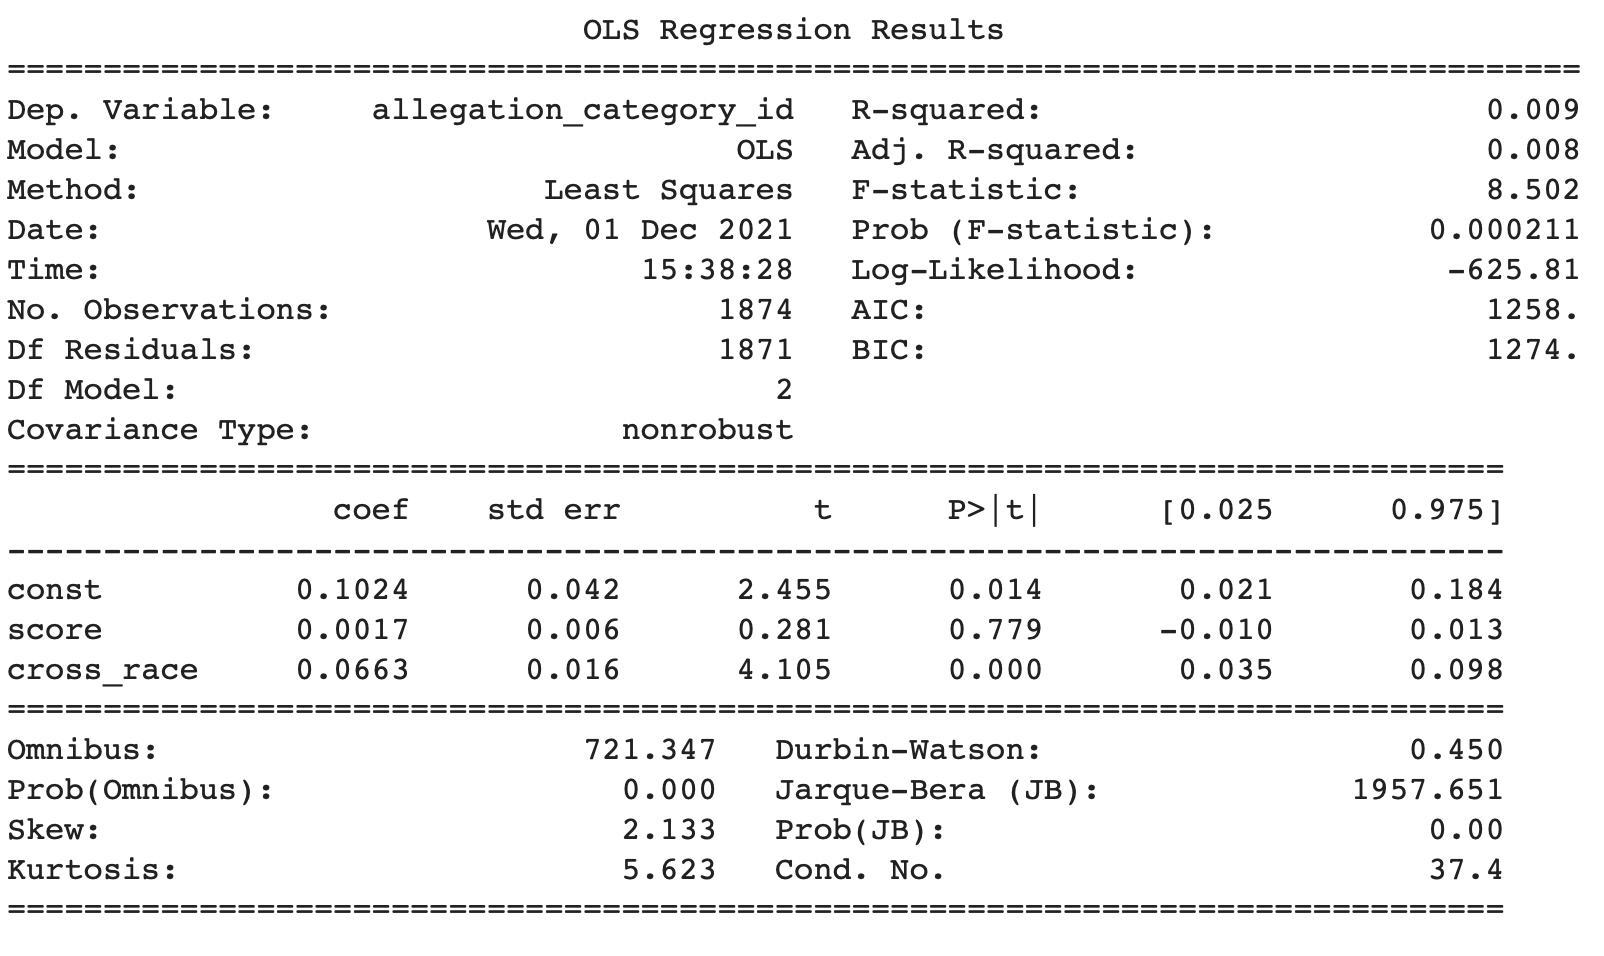
\includegraphics[width=\textwidth]{regression2}
\end{figure}

Distinguished from the first table, by combining the race of two parties, one can see from this table that being in different race groups with subjects is a statistically significant factor for officers to use force. 



\section{Conclusion}

We investigated the role race plays in police use of force by assessing the situation with a sentimental analysis and running regression analyses, controlling for the sentimental scores.
We discovered that being white is not necessarily a factor for police to use force but being black could be a factor that encourages police use of force. More importantly, police misconduct is evidently escalated if officers and subjects come from different race groups.

In this sense, one suggestion to reduce the excess and unfair use of force is that the police department should emphasize this conscious or unconscious bias towards people outside officers’ race groups in their internal training. The population could also react to police investigations more carefully, being aware of this bias.  



\section{Future direction}

We suspect that our sentimental scores did not show significance in regression because of the lack of first-hand complaint. The text we performed sentimental analysis on is third-party summaries that is rather neutral in reflecting the heat of the situations. This reduces the predicting power of the sentimental scores. In the future, researchers should attempt to obtain raw complaint texts.

Besides, we only investigated two allegations. In order to have a whole view of factors that go into the severity of police misconduct, researchers should attempt to rank all the allegations by their severity levels as their dependent variable in the regression analysis.



\end{document}
